\documentclass[11pt]{amsbook}
\usepackage[pdftex]{graphicx}
\usepackage{../HBSuerDemir}
\usepackage{wrapfig}
 

\begin{document}
% -------------------------------------------------------------------
\chapter{ANALYTIC GEOMETRIC IN $\mathbb{R}^3$}
\section{VECTORS}

% ++++++++++++++++++++++++++++++++++++++
\hPage{b2p1/117}
% ++++++++++++++++++++++++++++++++++++++
%\heading{ANALYTIC GEOMETRIC IN $\mathbb{R}^3$}

\begin{defn}
In Physical science are quantities such as velocity and acceleration that are determined not only by magnitude(length) but also by direction and sense. Such quantities have the common name vector. Vectors are very powerful tools in treating analytic geometry.
\end{defn}

%\end{definition}
\begin{wrapfigure}{r}{0.6\linewidth}
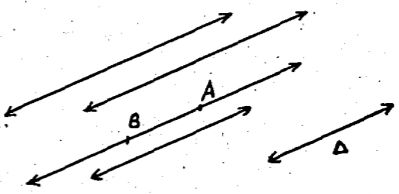
\includegraphics[width=\linewidth]{images/11}
\end{wrapfigure}

The set of all parallel lines in space define a direction, ${\Delta}$, and each line AB of the set has this indicated direction and defines two senses, one from A to B, the other from B to A.

A line segment [AB] with end points A and B has a direction (that of its support line), and a length $|AB|$.

A line segment [AB] oriented from one end to the other, say from A to B, is called a line vector, written $\ \overrightarrow{AB}$. A is the initial point or the point of application and B the extremity of $\ \overrightarrow{AB}$.


\begin{figure}[!htb]
\minipage{0.32\textwidth}
  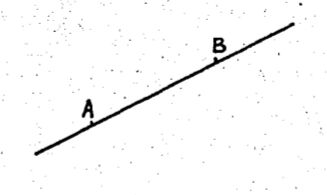
\includegraphics[width=\linewidth]{images/12.jpeg}
  \textbf{line AB (has a direction)}
\endminipage\hfill
\minipage{0.32\textwidth}
  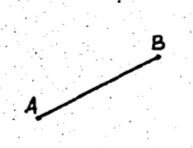
\includegraphics[width=\linewidth]{images/13.jpeg}
  \textbf{line segment [AB] (has a direction and length)}
\endminipage\hfill
\minipage{0.32\textwidth}%
  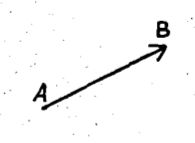
\includegraphics[width=\linewidth]{images/14.jpeg}
  \textbf{vector $\widehat{AB}$ (has a direction length and sense}
\endminipage
\end{figure}
\end{document}